\documentclass{article}
\usepackage[utf8]{inputenc}
\usepackage{graphicx}
\usepackage{amsmath}

\title{608 - Spectroscopy of Supernova 1987A}
\author{Massimiliano Lincetto, Patrik Veres, Nikolas Korzoun}
\date{April 2026}

\begin{document}

\maketitle

\section{Introduction}

During most of their existence, stars derive their radiated energy from the fusion of hydrogen into helium.
When the hydrogen supply is largely depleted, the star shrinks. 
This increases the pressure and temperature at its center and leads to the onset of helium burning, with carbon as the end product.
When the helium supply is also largely depleted, stars of solar size or smaller terminate their active phase, then shrink to planetary size, and finally burn out as white dwarfs.
The density reached in this process leads to the degeneracy of the electron gas, whose Fermi pressure balances gravity.
In stars of more than 6 times the mass of the Sun, the fusion chain is prolonged by carbon burning and other fusion processes until pressure and temperature in the stellar core are high enough to fuse silicon into iron.
However, the steadily growing iron core in the interior cannot supply any more energy by fusion, since energy is consumed to fuse nuclei heavier than iron.
When fusion is halted, the stellar core collapses in less than a tenth of a second.
During this process, temperature in the core is so high (3 $\times$ 10$^9$ K) that atoms are no longer stable.
They become decomposed into nucleons by high-energy $\gamma$-ray photons.
Furthermore, protons and electrons recombine by electron capture:
\begin{equation}
    e^{-} + p \to n + \nu
\end{equation}
The entire iron core is converted into neutrons, thereby forming a neutron star.
The neutrons, like electrons in a white dwarf, are Fermi-degenerate.
Their Fermi pressure stabilizes the nucleus.
For a brief moment during the collapse, the stellar core reaches a nucleon density greater than $10^{15}$\,kg\,m$^{-3}$.
Under these extreme conditions, the collapse is transformed into a shock wave that travels roughly 1000\,km\,s$^{-1}$ through the remaining layers of the star, tearing it apart.
Part of the energy is consumed to produce elements heavier than iron, but most of the energy from the collapse is released in the form of neutrinos.

After a few hours, the shock wave reaches the surface.
The surface is heated to over $10^5$\,K, and begins to glow.
At this stage, the collapsed star becomes visible as a supernova\footnote{There are two types of supernovae, each with different light curves and spectra. The core collapse described here leads to a type II supernova}.
The envelope continues to expand for a few thousand years until its density becomes low enough to be decelerated by the surrounding interstellar material.
A famous example is the Crab Nebula in Taurus.
Modern telescopes observe dozens of supernova explosions each year, but they are more commonly observed in distance galaxies, and are therefore very faint.
The last supernova in our own own Milky Way was observed by Johannes Kepler in 1604, a few years before the invention of the telescope. 
It was visible to the naked eye for a few weeks, and even in the daytime sky.

383 years later, on February 24, 1987, another supernova visible to the naked eye visible was detected in the Large Magellanic Cloud (LMC).
The LMC is our nearest neighboring dwarf galaxy, and is easily visible from the southern hemisphere.
A day earlier, neutrino detectors in Japan, the USA, and the USSR detected about two dozen neutrinos which had to originate from outside the solar system.
Their frequency, time, and energy distributions were compatible with the assumption that they originated from a supernova in the LMC.
The exact time of core collapse had been determined and, for the first time, neutrinos from outside our solar system had been detected.
Supernova 1987A (SN 1987A), as it is officially called, has been studied across the electromagnetic spectrum, from radio to $\gamma$-rays.
The evolution of its brightness and spectral profile had been measured with unprecedented precision and time coverage.
Numerical models for collapse and explosion were fit to the data, and our theoretical understanding of this important final phase of stellar evolution was decisively improved.

In this experiment, we will investigate the spectrum of SN 1987A.
You will measure the expansion velocities of its envelope, and estimate its distance on the basis of spectrophotometric data measured by the staff of the Astronomical Institute of the RUB.
This is largely done with computer-aided image processing, which has become a standard working tool in astronomy.
Therefore, the aim of this experiment is also to get to know these working methods.

\section{Experimental Data}
Absolutely calibrated fluxes, $F(\lambda,t)$ (in 10$^{-12}$\,J\,m$^{-2}$\,s$^{-1}$\,nm$^{-1}$) of SN 19S7A are available.
They were obtained with a spectrum scanner at the 61\,cm telescope of the Astronomical Institute of the RUB at the European Southern Observatory (ESO) site on La Silla.
The covered wavelength range is 320 -- 880\,nm, with a resolution of 1\,nm.
Selected spectra are shown in Figure \ref{fig:fig1}.
% The data are available as files on the Alpha computers (tag0002-tagOIOO), and the current path name can be obtained from your supervisor.
The experiment is evaluated with the image processing program MIDAS, which has been developed by ESO for astronomical image processing.
This image processing system is suitable for processing all kinds of one-dimensional (e.g. spectra) or two-dimensional (e.g. digitized sky images) data fields.
The user works with a number of commands, with which they can e.g. add data files, multiply them, display them on screen, or process them in other ways.
% The essential commands needed in the experiment are listed in the last section, and a manual and online help are also available.
% A workstation is reserved for the experiment from 10:30 on the day of the experiment.
The data you will be working with has been converted to Flexible Image Transport System (FITS) files, a standardized data format in astronomy.
FITS files can be analyzed in \texttt{python} (e.g. using packages like \texttt{astropy}).

\begin{figure}[p]
    \centering
    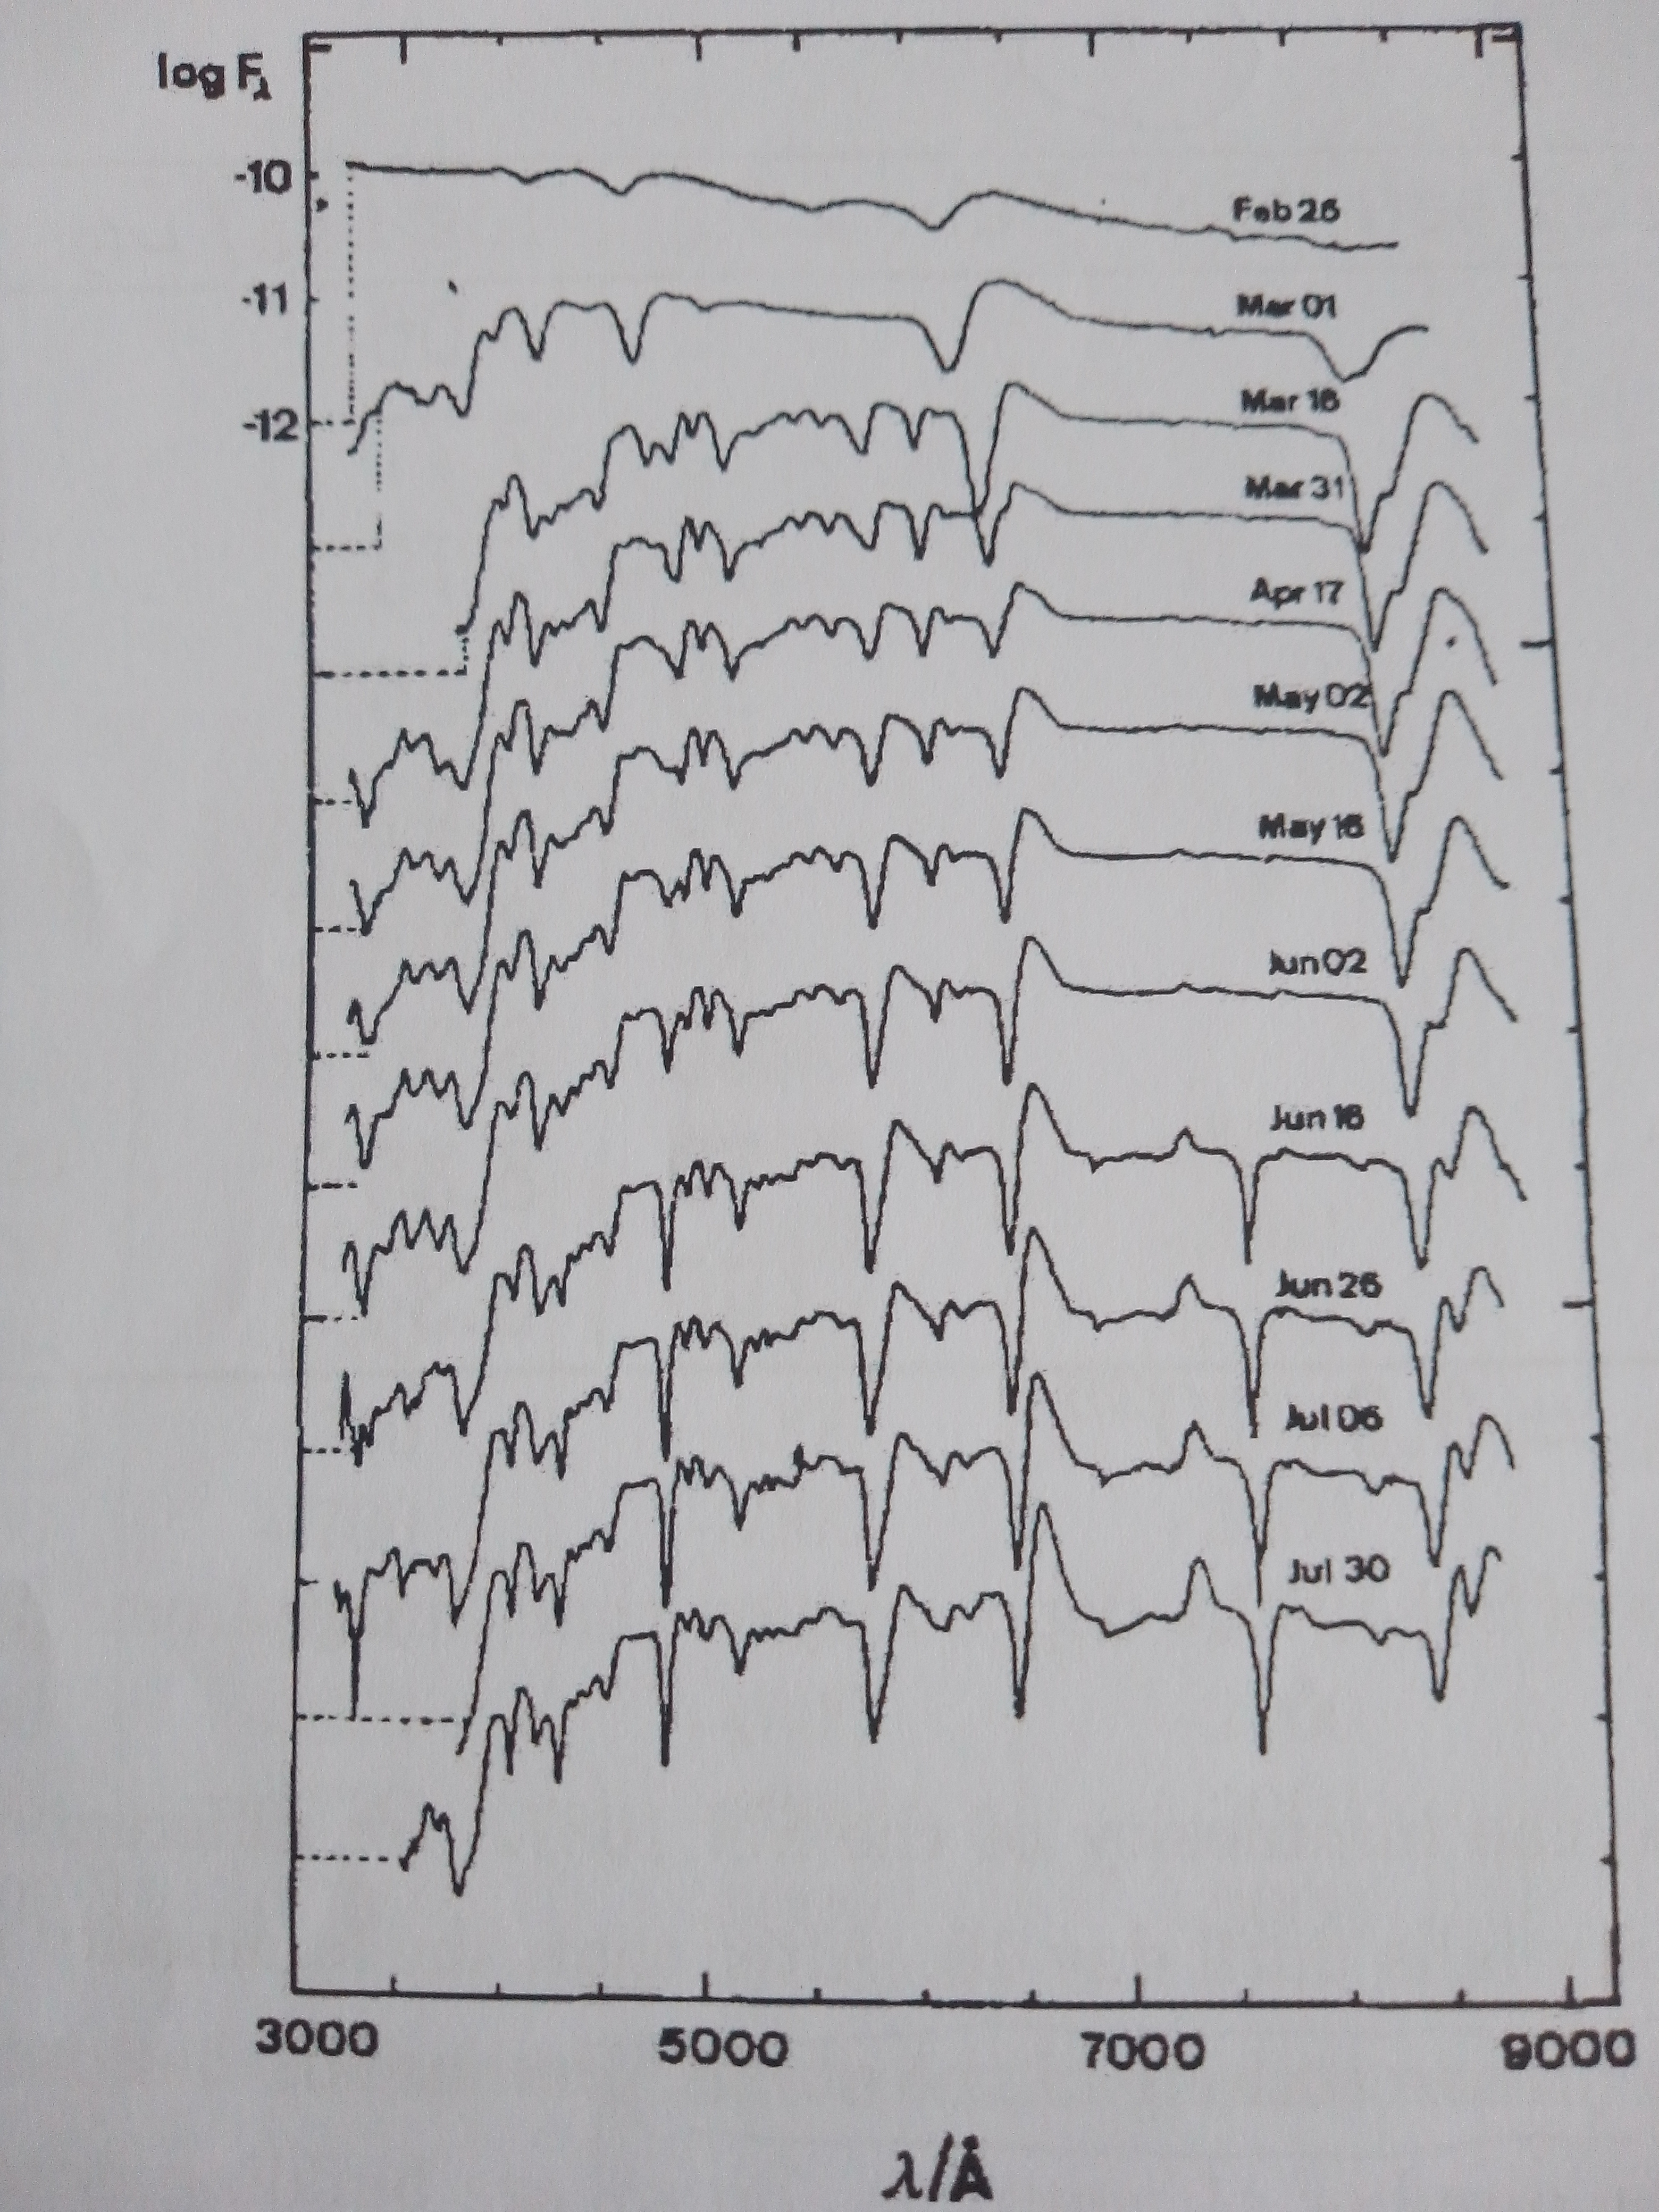
\includegraphics[width=0.8\textwidth]{inc/sp.jpg}
    \caption{Spectral evolution of SN 1987A. Logarithmically displayed are flux calibrated spectra from Bochum measurements on selected dates. The spectra are shifted downwards by one power of ten.}
    \label{fig:fig1}
\end{figure}

The data are calibrated to remove the effects of extinction in Earth's atmosphere by processes like scattering and absorption.
Their fluxes are also calibrated by measuring standard stars on the same night of each observation.
The spectral flux distribution of these standard stars are known in great detail from careful comparisons to primary standards (Vega, the Sun) and to lab furnaces (a good approximation of a black body).

\section{Identification of Spectral Lines}
The velocity field in the expanding supernova envelope resembles that of a terrestrial explosion; the outermost particles are the fastest.
Furthermore, the expansion, at least in the initial phase observed here, takes place unconstrained.
For a homologous expansion, where velocity is proportional to radius, it is then valid that
\begin{equation}
    v(r,t) = \frac{r}{t-t_0}
\end{equation}
where $t_0$ is the explosion time.
The envelope initially expands adiabatically and cools rapidly to approximately $10^4$\,K.

Apart from its high expansion velocity in the early phase, the envelope resembles a normal stellar atmosphere.
There exists an inner quasi-photosphere from which the continuum radiation originates, and a less dense outer layer (the atmosphere).
The continuum radiation in the photosphere originates from Thomson scattering of photons by free electrons.
It is this layer from which a photon has an appreciable probability of escape.
For an observer, it is the innermost layer that can still be seen; the layers at greater depth are not visible.

At certain wavelengths where strong absorption can occur, the absorption coefficient is several orders of magnitude larger than in the nearby continuum. 
Continuum radiation emerges from the photosphere at all angles, but radiation at these wavelengths is absorbed or scattered in the outer layer of gas.
An observer receives radiation only from photons traveling along the line of sight toward them.
Geometrically, the expanding envelope consists of two regions. 

First, there is a foreground region between the photosphere and the observer (along the line of sight). 
Photons from the photosphere at these absorption wavelengths must pass through this foreground gas. 
Since the absorption coefficient is very large, these photons are absorbed or scattered out of the line of sight before reaching the observer. 
The observer therefore measures a smaller flux of these photons than the surrounding continuum, an absorption line feature.

Second, there is the rest of the envelope (the regions off the line of sight).
Gas there absorbs photons from the photosphere at these wavelengths and scatters them in random directions.
Some of these scattered photons are redirected into the line of sight and reach the observer.
The observer therefore measures a greater flux of these photons than the surrounding continuum, an emission line feature.

The superposition of absorption from the foreground and emission from the rest of the envelope produces a characteristic P Cygni profile (named after the star where this type of profile was first studied in detail), shown schematically in Figure \ref{fig:fig2}.
The profile shows both an absorption dip (from the foreground) and an emission bump (from the rest of the envelope), with the relative strengths depending on the expansion velocity and density structure.
The wave velocities of the scattered or emitted line photons are Doppler shifted according to the relative velocity of the particles:
\begin{equation}
    \lambda - \lambda_0 = \lambda_0 \frac{v}{c},
\end{equation}
where $\lambda_0$ is the rest wavelength, $v$ is the velocity, and $c$ is the speed of light in vacuum.

\begin{figure}[tb]
    \centering
    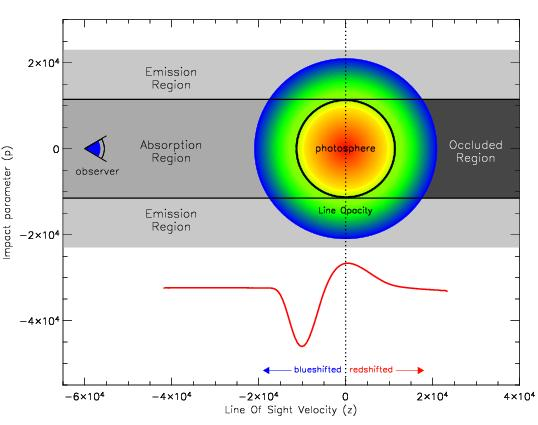
\includegraphics[width=0.8\textwidth]{inc/pline.jpg}
    \caption{Schematic description of the P Cygni profile.}
    \label{fig:fig2}
\end{figure}

\subsection{Tasks}
Using the SN spectrum measured on different days (e.g., days 2, 10, and 50) after the explosion:
\begin{itemize}
    \item How does the spectrum change (brightness, flux distribution, etc...)?
    \item Where do you see continuum radiation?
    \item Where do you see absorption lines?
    \item Where do you see emission lines?
    \item What elements/ionization levels do you expect to see in the spectrum?\footnote{Hint: SN 1987A was a Type II supernova with hydrogen in the envelope. The spectrum of a 5500\,K supernova envelope is similar to that of a G star, e.g. the Sun.}
    \item How large are the radial velocities typically?
\end{itemize}

\section{Radial Velocities}
The laws governing supernova expansion are known quite well.
It is possible, given a velocity of the spherical shell, to determine its radius at any given time.
However, it is not possible to determine the absolute velocity from the spectrum alone.
Only the radial component of the velocity can be inferred from spectroscopic measurements through Doppler shifts.
Converting measured line shifts into physical radii is not straightforward.

A single spherical shell with expansion velocity $v_\text{exp}$ contributes to the P Cygni profile over a range of radial velocities, with the most blueshifted\footnote{By convention, blueshifted velocities, moving toward the observer, are negative. Redshifted velocities, moving away from the observer, are positive.} contribution at $v_\text{rad} = -v_\text{exp}$.
In principle, parts of each spherical shell in the envelope contribute to the line absorption, and these contributions are smeared over a certain radial velocity range.
The observer therefore sees only the net effect integrated throughout the envelope.
However, the density gradient in the envelope is very steep ($N \sim r^{-7...-10}$).
Therefore, the layer at which the optical depth $\tau$ reaches 1 is sharply defined.
The optical depth at point $r$ in the envelope along a line of sight is given by:
\begin{equation}
    \tau(r) = \int_{-\infty}^{r} \kappa N(r')\,dr'
\end{equation}
where $N$ is the number density of absorbing particles, and $\kappa$ is the line absorption coefficient.
The wavelength of the absorption minimum is first converted into the velocity $v_\text{abs}$ by the Doppler shift.
Thus, at some radius $r_\text{abs}$, maximum absorption takes place ($\tau = 1$), and this radius corresponds to the measured velocity $v_\text{abs}$ of the absorption minimum in a spectral line:
\begin{equation}
    r_\text{abs} = v_\text{abs}\,(t - t_0)
    \label{eq:r_abs}
\end{equation}
The radius $r_\text{abs}$ will be close to the photosphere for weak lines, i.e. those where one can look deep into the envelope. 
For strong lines, however, $r_\text{abs}$ will be reached farther out.

\subsection{Task}
For days 2, 5, 10, 20, 30, ... 100, determine the radial velocities of the absorption minimum of the following lines:
\begin{itemize}
    \item $H_\alpha$, $\lambda=6563$\,\AA
    \item Na I-D, $\lambda=5890$\,\AA
    \item Ba II-2, $\lambda=6141$\,\AA
    \item Fe II-42, $\lambda=5018$\,\AA
\end{itemize}
Note: not all lines are already seen on day 2.
Using Equation \ref{eq:r_abs}, convert these values into spectroscopic radii $r_{\text{abs}}$ in units of solar radii, $R_\odot=6.96\times 10^8$\,m.
Discuss reasons for the stratification found.

\section{Photosphere radius and distance to SN~1987A}
The determination of the effective radius $r_{\text{abs}}$ of the maximum absorption of various lines is a distance-independent radius determination of the envelope.
Only the Doppler effect plays a role here.
A second method of radius determination is distance dependent.
The bolometric (total) luminosity of a star, or an expanding gas sphere, is given by the Stefan-Boltzmann Law:

\begin{equation}
    L = 4 \pi r_{\text{ph}} \sigma T^4_{\text{eff}}
    \label{eq:stefan-boltzmann}
\end{equation}

Therefore, the photospheric radius $r_{ph}$ can be determined from a known luminosity and temperature.
This photospheric radius corresponds to the layer from which the continuum radiation escapes, and is therefore less than or equal to the above determined radii of the line-absorbing layers.
The temperature of a supernova can be determined in a few ways: by fitting a blackbody to the observed energy distribution, by using the wavelength of the continuum maximum to estimate a Wien temperature, or by fitting numerical models to the data. 
The last method is the most accurate, but also by far the most computationally demanding.
The bolometric luminosity $L$ is obtained from an integration over the measured flux in the UV, optical, and infrared at a known distance $D$. 
Contributions from other wavelength ranges can be neglected.
\begin{equation}
    L_D(t) = 4 \pi D^2 \int_0^{+\infty} F(\lambda,t) d\,\lambda
\end{equation}

Numerical values for the luminosity of SN~1987A from photometric data are listed in Table \ref{tab:l_bol} for some selected days.
The supernova's radiation is reddened on its way to the observer by interstellar dust in the LMC and in our own Milky Way.
Photons get scattered in a wavelength-dependent manner, and the measured flux must be corrected for this interstellar extinction.
The luminosity values in Table \ref{tab:l_bol} were calculated under the assumption that the supernova is at D = 50\,kiloparsec (1\,parsec = 3.1 $\times$ 10$^{16}$\,m), the distance to the LMC.
The exact distance to the supernova is not determined, so the values in Table \ref{tab:l_bol} must be scaled.
\begin{equation}
    L_D(t) = L_{50}(t)\,(D/50\,\text{kpc})^2
\end{equation}
The true distance $D$ of the supernova can be determined by comparing the spectroscopic radius $r_\text{abs}$ from Equation \ref{eq:r_abs} with the photospheric radius $r_\text{ph}$ from Equation \ref{eq:stefan-boltzmann}.
This method of distance determination (analagous to the Baade-Wesselink method) is an essential pillar in the determination of cosmic distances.

\clearpage
\subsection{Tasks}
\begin{itemize}
    \item Determine the effective temperature of the supernova envelope for the days given in Table \ref{tab:l_bol}.
    You should use the provided Planck curves (pla0001 - pla0016) for this, which you multiply by a suitable scaling factor and fit on the screen.
    As a second method, determine the approximate maximum of the continuum radiation, and use it to calculate the Wien temperature of the supernova envelope using Wien's displacement law.
    Discuss the advantages and disadvantages of both methods.
    \item From the effective temperature, calculate the radius of the photosphere for the days indicated using the values of the luminosity $L_{50}$ in Table \ref{tab:l_bol}.
    \item Compare these radii with spectroscopic radii $r_\text{abs}$ (Equation \ref{eq:r_abs}), from the above mentioned FeII and BA II lines (why these?) and determine the true distance D of the supernova 1987A from a possibly necessary scaling.
    \item Estimate how much energy SN 1987 A emitted as electromagnetic radiation in the first 100 days, and compare this amount with the kinetic energy of the ejected shell ($v \approx 10^4$\,km\,s$^{-1}$, $M \approx 10\,M_\odot$ = $2 \times 10^{31}$\,kg) and the energy of the neutrino pulse which was released during the collapse\footnote{Hint: the IMB detector in the USA (surface approx. 20\,x\,20\,m$^2$, efficiency $\eta \approx 6 \times 10^{-16}$) detected a total of 8 neutrinos with 30\,MeV each.}.
    Discuss the result.
\end{itemize}

\clearpage
\begin{table}[htb]
    \caption{Bolometric luminosity $L_{50}$ of SN 1987A. (From Catchpole et al. 1987, MNRAS, 229, 15P)}
    \vspace{0.2cm}
    \centering
    \begin{tabular}{c|c}
         Day since 23 Feb 1987 & log $L_{50}$ / LSun \\ \hline
         2 & 8.06 \\
         5 & 7.77 \\
        10 & 7.73 \\
        20 & 7.86 \\
        30 & 7.97 \\
        40 & 8.09 \\
        50 & 8.20 \\
        70 & 8.35 \\
       100 & 8.34 \\
    \end{tabular}
    
    \label{tab:l_bol}
\end{table}

\begin{table}[htb]
    \caption{Provided Planck curves}
    \vspace{0.2cm}
    \centering
    \begin{tabular}{c|c}
        File & Temperature [K]  \\ \hline
        pla0001 & 5000 \\
        pla0002 & 5500 \\
        pla0003 & 6000 \\
        ... & ... \\
        pla0011 & 10000 \\
        pla0012 & 11000 \\
        pla0013 & 12000 \\
        pla0014 & 13000 \\
        pla0015 & 14000 \\
        pla0016 & 15000 \\
    \end{tabular}
\end{table}

\end{document}
